\pagebreak
\chapter[Introduction]{}\vspace{-2cm}\noindent\rule{\textwidth}{2.5pt}
\thispagestyle{empty}

\vspace{5cm}\textbf{\huge{Introduction}}

\medskip\noindent\rule{\textwidth}{1pt}

As NASA prepares to return to the Moon, innumerable activities to equip, shelter, and otherwise support future astronauts are underway.  These astronauts will be eating and drinking, and subsequently urinating and defecating in microgravity and lunar gravity.  While astronauts are in the cabin and out of their spacesuits, they will need a toilet that has all the same capabilities as ones here on Earth. NASA is calling on the global community for their novel design concepts for compact toilets that can operate in both microgravity and lunar gravity.  These designs may be adapted for use in the Artemis lunar landers that take us back to the Moon.  Although space toilets already exist and are in use (at the International Space Station, for example), they are designed for microgravity only.  NASA’s Human Landing System Program is looking for a next-generation device that is smaller, more efficient, and capable of working in both microgravity and lunar gravity. This challenge includes a Technical category and Junior category.

\pagebreak
It is in this calling of this unique challenge that we wish to provide a solution that is both functional and innovative. This document will provide our design rationale, the functionality of the product, and how this design has innovated prior designs.  

\section[Space Waste Collection Systems]{Overview of Space Waste Collection Systems}
Space Waste Collection Systems(WCS) are the implementation of Earth toilets in a microgravity environment. However, easier said than done while in microgravity there poses a challenge of transporting and storing human waste. While in microgravity, fluids are pulled together through its surface tension causing the mundane task of transporting anything through a fluid system a non-trivial task. As a result of this non-trivial task, this seemingly simple task on Earth becomes a very intensive engineering project that cannot be overlooked.


    \subsection{Apollo Waste Collection System}

    During the age of Apollo, minimal work went into designing an effective waste collection system resulting from the difficulty of even obtaining a low Earth orbit. As a result the astronauts on-board would collect and dump urine overboard instead of storing the urine. 

    However, collecting urination from the astronauts was simple enough, collecting fecal matter is what proved to be most difficult. In order to avoid the troubles of defecating in space, many astronauts while in space would eat less of their rations to avoid the troubles of defecating in microgravity.

    \begin{quote}
        In the absence of a system providing positive means for the removal of feces from the body, an extremely basic system had to be relied upon for inflight fecal collection. The device used was a plastic bag which was taped to the buttocks to capture feces. After defecation, the crew member was required to seal the bag and knead it in order to mix a liquid bactericide with the contents to provide the desired degree of feces stabilization. Because this task was distasteful and required an inordinate amount of time, low residue foods and laxatives were generally used prior to launch. During flight, in addition to low residue foods, some use was also made of drugs to reduce intestinal motility.\cite{apollo_bathroom}
    \end{quote}

    \pagebreak

    \begin{figure}[h]
        \centering
        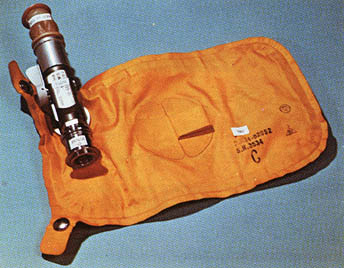
\includegraphics[width = 0.5\linewidth]{figs/apollo_urine_bag.jpg}
        \caption[Apollo Urine Transfer System]{Apollo urine transfer system.}
        \label{fig:apollo_urine_bag}
    \end{figure}

    Above in Figure \ref{fig:apollo_urine_bag} in which it had two main purposes: 1) dumping during time of voiding, and 2) dumping subsequent to voiding.

    \begin{figure}[h]
        \centering
        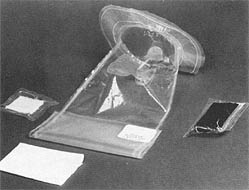
\includegraphics[width = 0.5\linewidth]{figs/apollo_fecal_bag.jpg}
        \caption[Apollo Fecal Bag]{Apollo fecal bag for defecating in microgravity.}
        \label{fig:apollo_fecal_bag}
    \end{figure}

    As shown above in Figure \ref{fig:apollo_fecal_bag}, the bag used to collect astronaut defecation's was rudimentary in design resulting in many of the astronauts being in great discomfort when defecating. This bag was placed over the anus of the astronaut, and would be sealed after use to prevent the spread of bacteria and pathogens.
    


    \pagebreak
    \subsection{Space Shuttle's Waste Collection System}

    \subsection{Soyuz Waste Collection System}

    \subsection{International Space Station Waste Collection System}

    Test \cite{iss_background}

 
    \pagebreak
    
    \printbibliography[type=article,title = {References}, heading=subbibintoc]
    {\vspace{-2cm}\vskip-\ht\strutbox\makebox[\textwidth][c]{\rule{\dimexpr\textwidth}{2pt}}\par}

    \thispagestyle{empty}


